\chapter{Дерево рішень}\label{cha:decision_tree}
Ми використовуємо дані, щоб вирішити, як \underline{розбити} будинки на дві (див. Малюнок 1) \underline{групи}, а потім знову визначити прогнозовану ціну в кожній групі.
Цей етап фіксації шаблонів з даних називається \textbf{пристосуванням} або \textbf{навчанням} моделі.
Дані, що використовуються, щоб \textbf{відповідати} моделі, називаються \textbf{навчальними даними}.

Ви можете вловити більше факторів, використовуючи дерево, яке має більше «розбиттів».
Вони називаються \textbf{"глибшими" деревами}.
Дерево рішень, яке також враховує загальний розмір ділянки кожного будинку, може виглядати як на зображенні 2.

Прогнозована ціна на будинок знаходиться внизу дерева.
Точка внизу, де ми робимо прогноз, називається \textbf{листом}.

\begin{figure}
    \label{fig:image2}
    \centering
    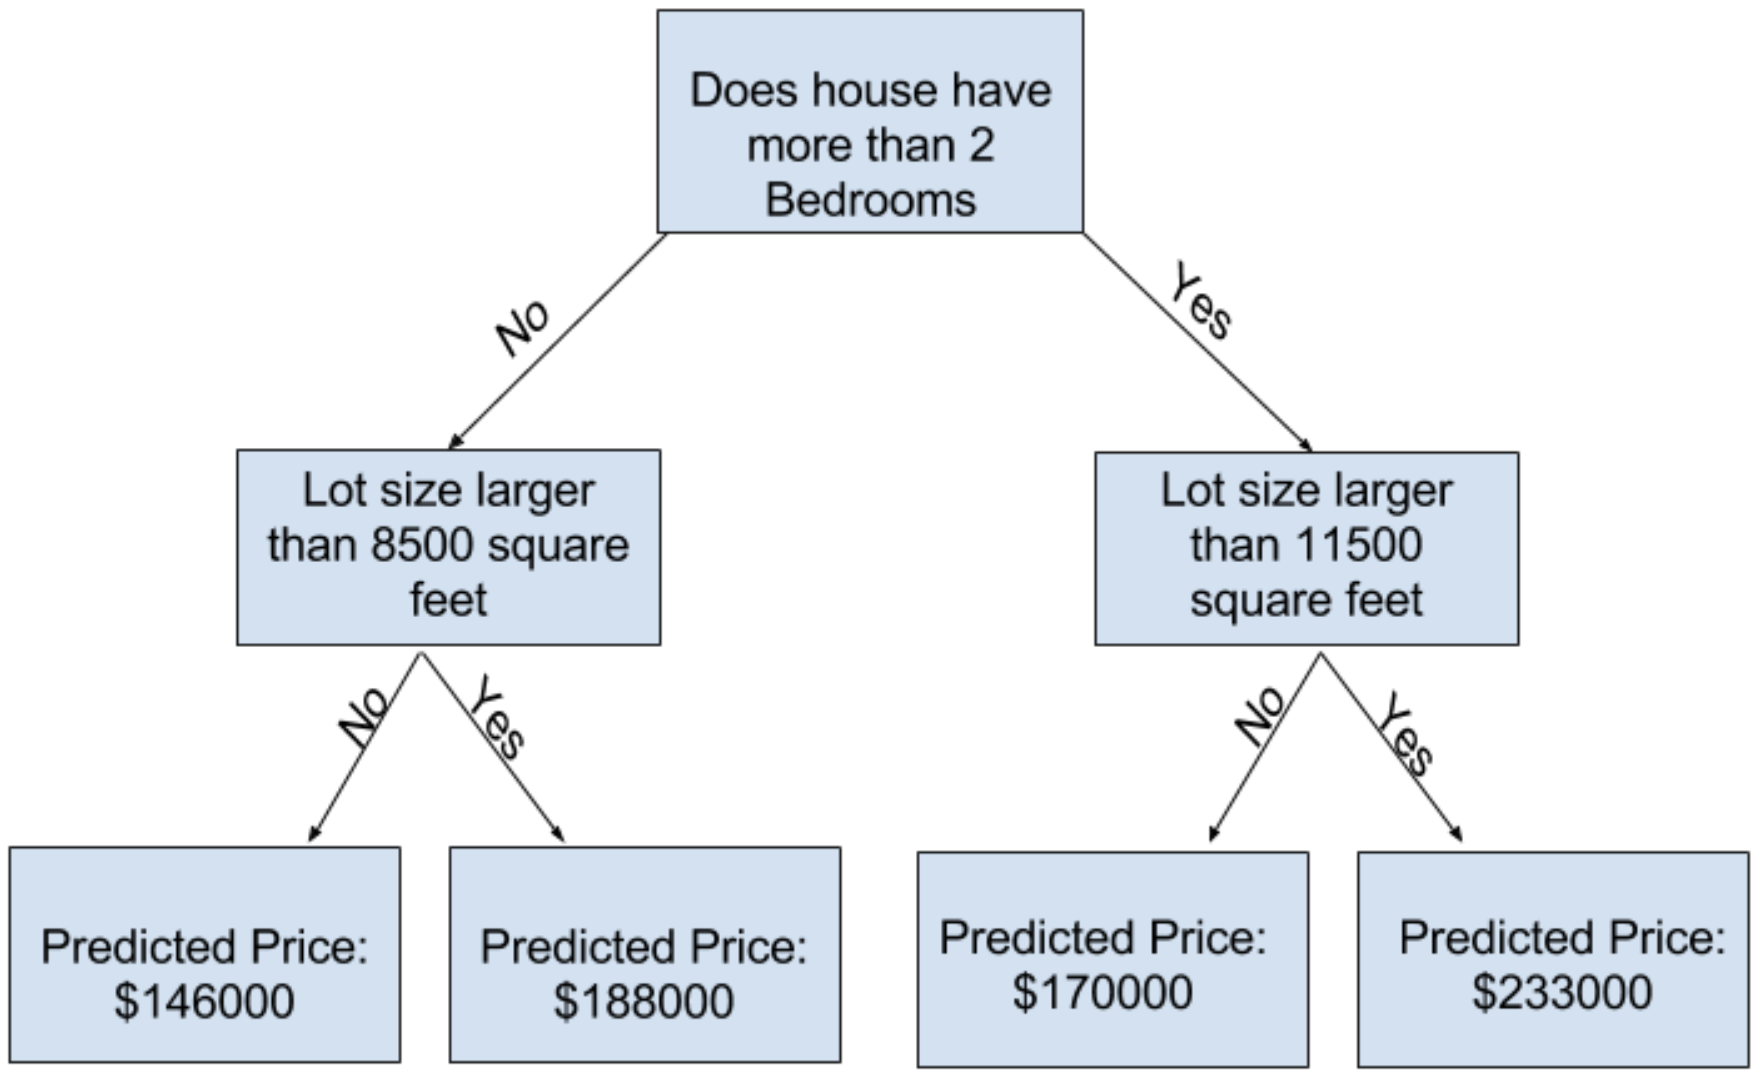
\includegraphics[scale=0.5]{image2.png}

    Deeper Trees
\end{figure}
